%%%%%%%%%%%%%%%%%%%%%%%%%%%%%%%%%%%%%%%%%%%%%%%%%%%%%%%%%%%%%%%%%%%%%%%%%%%%%%%%%%
\begin{frame}[fragile]\frametitle{}
\begin{center}
{\Large Conclusions}

\end{center}
\end{frame}


%%%%%%%%%%%%%%%%%%%%%%%%%%%%%%%%%%%%%%%%%%%%%%%%%%%%%%%%%%%
\begin{frame}[fragile]\frametitle{Conclusions}
\begin{itemize}
\item Graph-based Knowledge Graphs enhance LLMs in the enterprise context.
\item Leveraging Knowledge Graphs improves AI accuracy and relevance.
\item Benefits: Better data comprehension, refined compliance procedures, accelerated research and development.
\item CIOs should explore applying LLMs to internal data stores and constructing knowledge graphs using graph data science algorithms for substantial business breakthroughs.data science algorithms, as this strategy could yield substantial breakthroughs for their businesses.
\end{itemize}
\end{frame}

%%%%%%%%%%%%%%%%%%%%%%%%%%%%%%%%%%%%%%%%%%%%%%%%%%%%%%%%%%%%%%%%%%%%%%%%%%%%%%%%%%
%%%%%%%%%%%%%%%%%%%%%%%%%%%%%%%%%%%%%%%%%%%%%%%%%%%%%%%%%%%
\begin{frame}[fragile]\frametitle{Benefits of Combining Knowledge Graphs and LLMs}

\begin{itemize}
\item LLMs:
	\begin{itemize}
	\item  Hallucinate.
	\item   Have general knowledge.
	\item   Understand natural language.
	\item   Do not provide structured responses.
	\end{itemize}

\item KGs:
	\begin{itemize}
	\item   Do not understand language.
	\item   Provide structured responses.
	\item   Are accurate and interpretable.
	\item   Have domain-specific knowledge.
	\end{itemize}

\item LLMs+KGs have the potential to overcome some of the weaknesses of LLMs.

\end{itemize}

{\tiny (Ref: LinkedIn post by Miguel Fierro)}


\end{frame}

%%%%%%%%%%%%%%%%%%%%%%%%%%%%%%%%%%%%%%%%%%%%%%%%%%%%%%%%%%%
\begin{frame}[fragile]\frametitle{Benefits of Combining Knowledge Graphs and LLMs}

\begin{center}
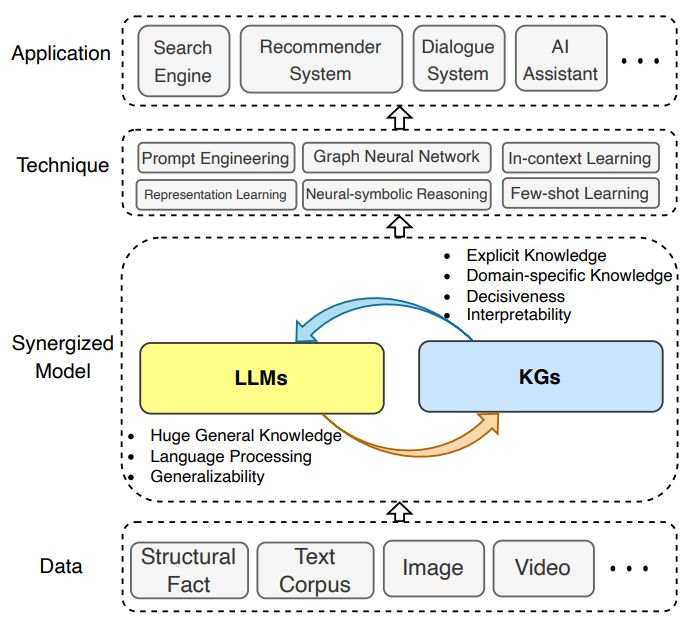
\includegraphics[width=0.6\linewidth,keepaspectratio]{llm54}
\end{center}	

{\tiny (Ref: LinkedIn post by Miguel Fierro)}

	
\end{frame}

%%%%%%%%%%%%%%%%%%%%%%%%%%%%%%%%%%%%%%%%%%%%%%%%%%%%%%%%%%%
\begin{frame}[fragile]\frametitle{Awesome-LLM-KG Github repo}

\begin{center}
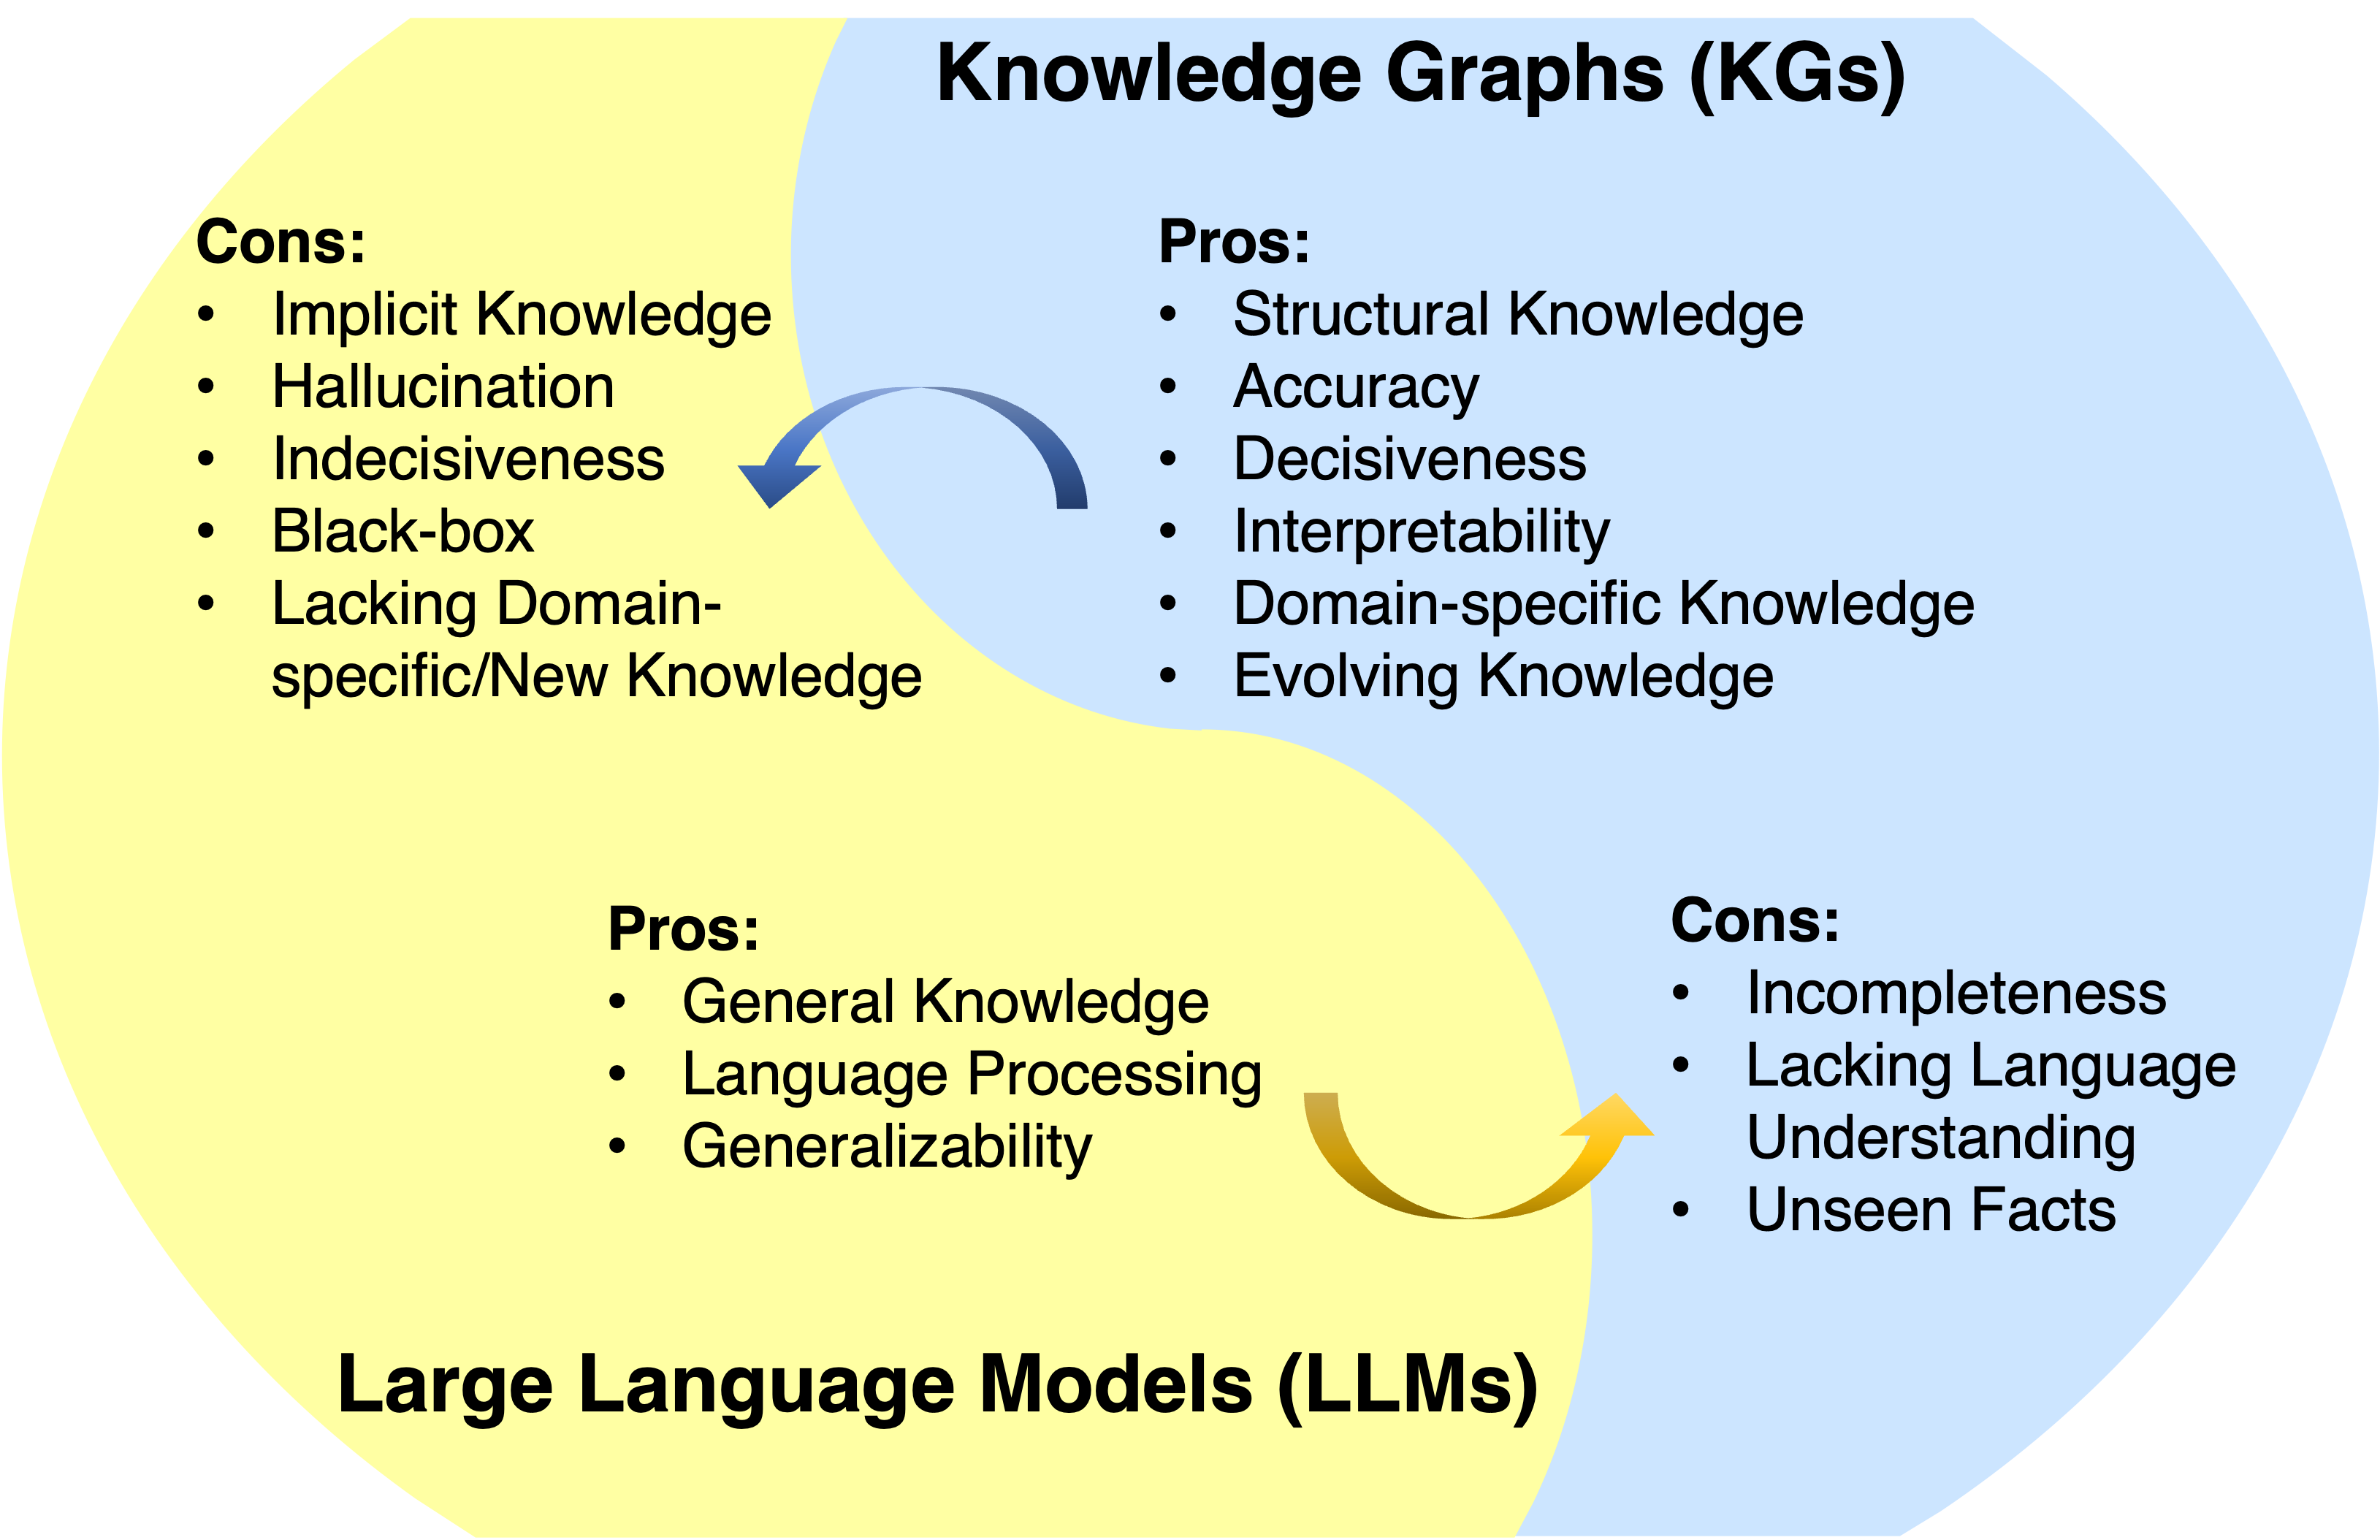
\includegraphics[width=0.8\linewidth,keepaspectratio]{llm55}
\end{center}	

{\tiny (Ref: https://github.com/RManLuo/Awesome-LLM-KG)}

	
\end{frame}

%%%%%%%%%%%%%%%%%%%%%%%%%%%%%%%%%%%%%%%%%%%%%%%%%%%%%%%%%%%
\begin{frame}[fragile]\frametitle{Awesome-LLM-KG Github repo}

\begin{center}
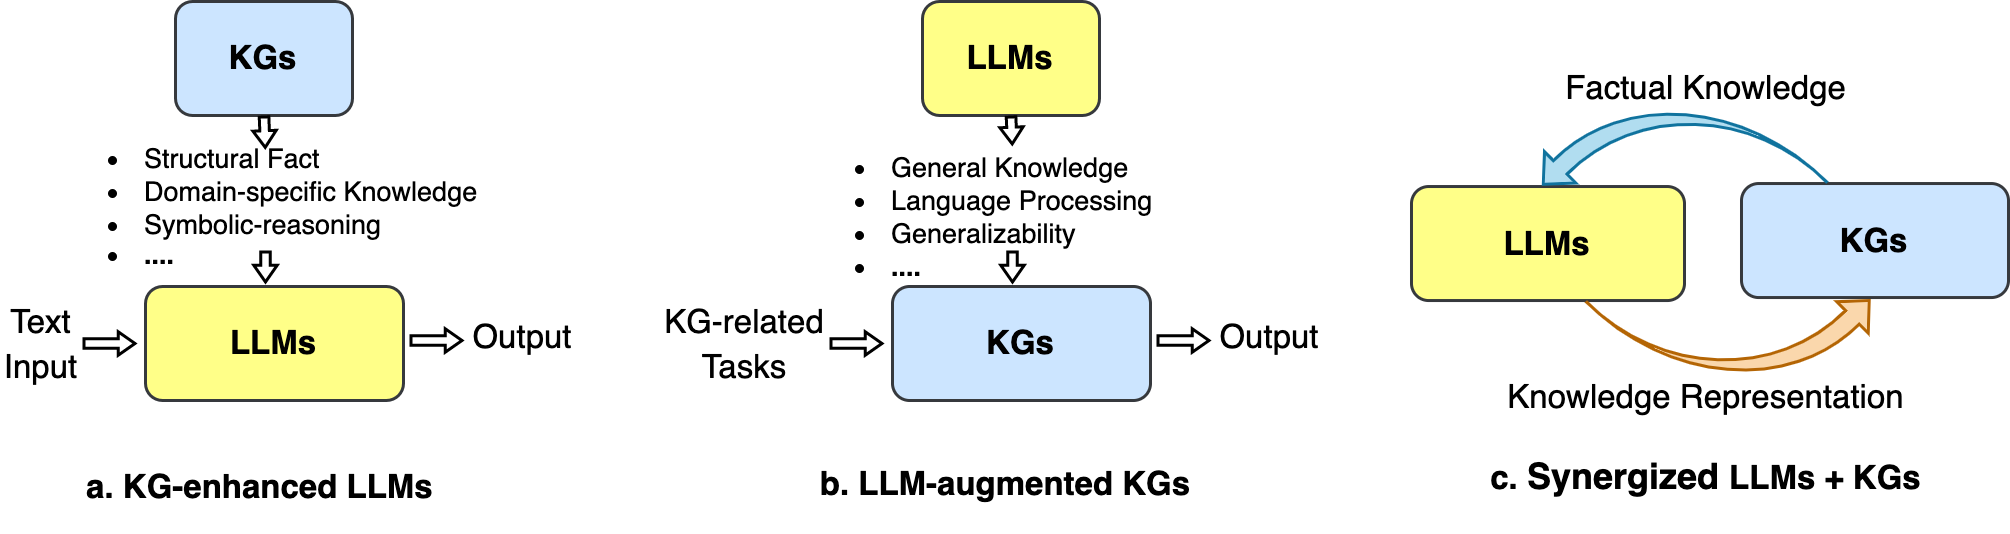
\includegraphics[width=\linewidth,keepaspectratio]{llm56}
\end{center}	

{\tiny (Ref: https://github.com/RManLuo/Awesome-LLM-KG)}

	
\end{frame}



%%%%%%%%%%%%%%%%%%%%%%%%%%%%%%%%%%%%%%%%%%%%%%%%%%%%%%%%%%%%%%%%%%%%%%%%%%%%%%%%%%
%%%%%%%%%%%%%%%%%%%%%%%%%%%%%%%%%%%%%%%%%%%%%%%%%%%%%%%%%%%
\begin{frame}[fragile]\frametitle{Benefits of Combining Knowledge Graphs and LLMs}

\begin{itemize}
\item Centralized source of accurate knowledge
\item Structured knowledge fusion of information in different formats
\item Increased informative value of collected data
\item Gives LLMs a human reference frame of the real-world
\end{itemize}

\end{frame}



% %%%%%%%%%%%%%%%%%%%%%%%%%%%%%%%%%%%%%%%%%%%%%%%%%%%%%%%%%%%
% \begin{frame}[fragile]\frametitle{Summary}

% Unifying Large Language Models \& Knowledge Graphs To Maximize Their Strengths \& Address Their Weaknesses

% \begin{center}
% 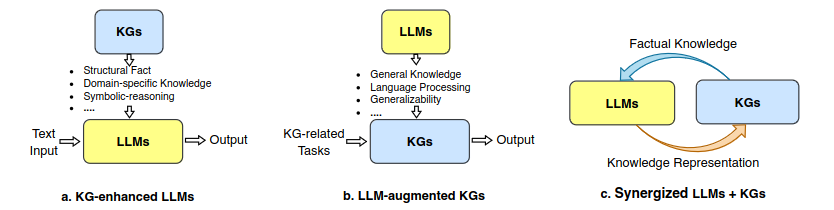
\includegraphics[width=\linewidth,keepaspectratio]{llm101}
% \end{center}	

% {\tiny (Ref: Combining Large Language Models and Knowledge Graphs - Haziqa Sajid )}

% \end{frame}


%%%%%%%%%%%%%%%%%%%%%%%%%%%%%%%%%%%%%%%%%%%%%%%%%%%%%%%%%%%%%%%%%%%%%%%%%%%%%%%%%%
%%%%%%%%%%%%%%%%%%%%%%%%%%%%%%%%%%%%%%%%%%%%%%%%%%%%%%%%%%%
\begin{frame}[fragile]\frametitle{What's next \ldots}

\begin{itemize}
\item Chain of Thought:
	\begin{itemize}
	\item LLM determines necessary steps
	\item Executes them sequentially
	\end{itemize}
	
\item Tree of Thought:
	\begin{itemize}
	\item Combines thought with symbolic tree search algorithm
	\item Enables optimal 'thought path' selection
	\item Advances LLM's planning complexity
	\end{itemize}
	
\item Graph of Thought:
	\begin{itemize}
	\item Thoughts modeled as nodes connected by edges
	\item Directed Acyclic Graphs (DAGs) used
	\item Revolutionizes data pipeline orchestration
	\item Models dependencies without circular loops
	\end{itemize}
	
\end{itemize}

{\tiny (Ref: LinkedIn post by Tony Seale)}

\end{frame}

%%%%%%%%%%%%%%%%%%%%%%%%%%%%%%%%%%%%%%%%%%%%%%%%%%%%%%%%%%%
\begin{frame}[fragile]\frametitle{What's next \ldots}

\begin{center}
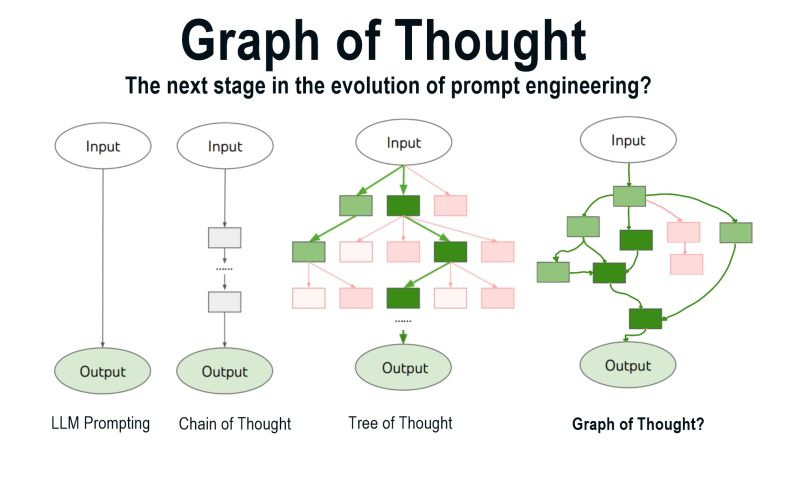
\includegraphics[width=\linewidth,keepaspectratio]{llm53}
\end{center}	

{\tiny (Ref: LinkedIn post by Tony Seale)}

	
\end{frame}



